% \begin{figure}[!t]
% \centering
% %   
\includegraphics[width=\columnwidth]{image/teaser} 
% 
\includegraphics[width=\columnwidth]{BLIPv2/image/fig1.pdf}
% \vspace{-3.5ex}
% \caption{Overview of BLIP-2 framework.
% \name~bootstraps vision-language pre-training from a frozen image encoder and a frozen LLM.
% }
% \vspace{-1ex}
% \label{fig:teaser}
% \end{figure}


% \begin{figure}[!t]
% \centering
% %   
\includegraphics[width=\columnwidth]{image/teaser} 
% 
\includegraphics[width=\columnwidth]{BLIPv2/image/fig1-minimal.pdf}
% \vspace{-3.5ex}
% \caption{Overview of BLIP-2 framework.
% \name~bootstraps vision-language pre-training from a frozen image encoder and a frozen LLM.
% }
% \vspace{-1ex}
% \label{fig:teaser}
% \end{figure}

\begin{figure}[!t]
\centering
%   
\includegraphics[width=\columnwidth]{image/teaser} 
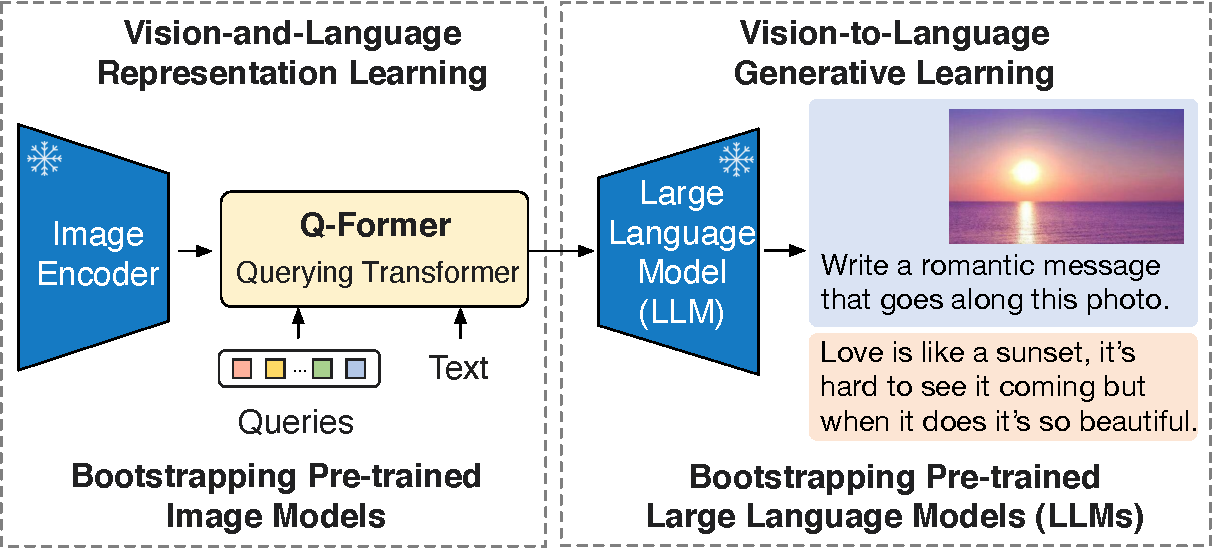
\includegraphics[width=1\columnwidth]{image/fig1-example.pdf}
\vspace{-3.5ex}
\caption{Overview of BLIP-2's framework.
We pre-train a lightweight Querying Transformer following a two-stage strategy to bridge the modality gap.
The first stage bootstraps vision-language representation learning from a frozen image encoder.
The second stage bootstraps vision-to-language generative learning from a frozen LLM,
which enables zero-shot instructed image-to-text generation (see Figure~\ref{fig:example} for more examples).}
\vspace{-2.5ex}
\label{fig:teaser}
\end{figure}
